\documentclass{standalone}
\usepackage{pgfplots}
\usepackage{amsmath}

\begin{document}
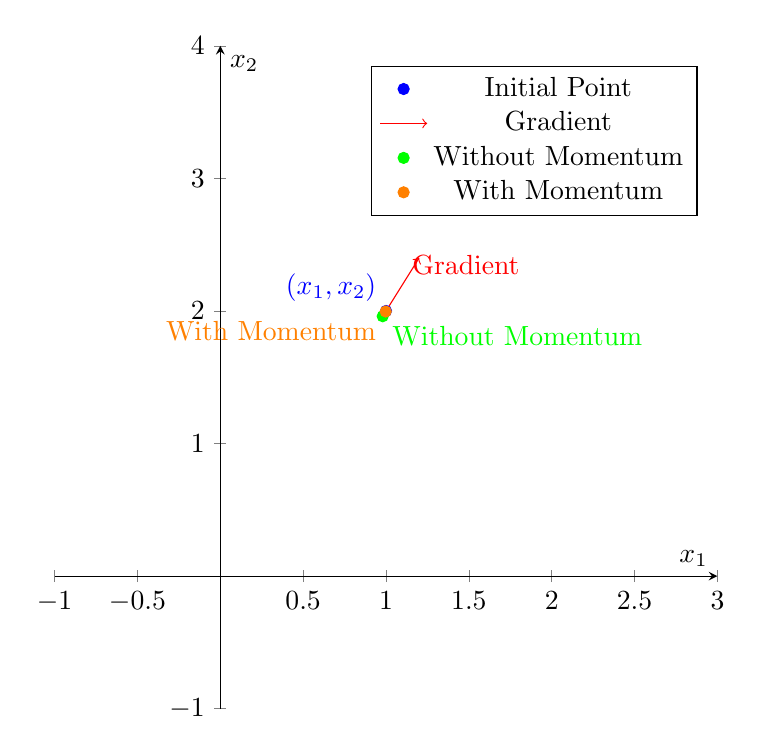
\begin{tikzpicture}
  \begin{axis}[
      axis lines = middle,
      xlabel = {$x_1$},
      ylabel = {$x_2$},
      xmin = -1, xmax = 3,
      ymin = -1, ymax = 4,
      width=10cm,
      height=10cm,
      legend pos=north east
    ]
    % Parameters
    \pgfmathsetmacro{\xone}{1}
    \pgfmathsetmacro{\xtwo}{2}
    \pgfmathsetmacro{\gradxone}{2*\xone}
    \pgfmathsetmacro{\gradxtwo}{2*\xtwo}
    \pgfmathsetmacro{\alpha}{0.01}
    \pgfmathsetmacro{\beta}{0.9}

    % Compute new points
    \pgfmathsetmacro{\xoneNew}{\xone - \alpha * \gradxone}
    \pgfmathsetmacro{\xtwoNew}{\xtwo - \alpha * \gradxtwo}

    % Compute new points with momentum
    \pgfmathsetmacro{\voneNew}{\beta * 0 + (1 - \beta) * \gradxone}
    \pgfmathsetmacro{\vtwoNew}{\beta * 0 + (1 - \beta) * \gradxtwo}
    \pgfmathsetmacro{\xoneNewMomentum}{\xone - \alpha * \voneNew}
    \pgfmathsetmacro{\xtwoNewMomentum}{\xtwo - \alpha * \vtwoNew}

    % Plot initial point
    \addplot[only marks, mark=*, blue] coordinates {(\xone, \xtwo)} node[above left] {$(x_1, x_2)$};

    % Plot gradient direction
    \addplot[red, ->] coordinates {(\xone, \xtwo) (\xone + \gradxone/10, \xtwo + \gradxtwo/10)} node[midway, above right] {Gradient};

    % Plot updated point without momentum
    \addplot[only marks, mark=*, green] coordinates {(\xoneNew, \xtwoNew)} node[below right] {Without Momentum};

    % Plot updated point with momentum
    \addplot[only marks, mark=*, orange] coordinates {(\xoneNewMomentum, \xtwoNewMomentum)} node[below left] {With Momentum};

    \legend{Initial Point, Gradient, Without Momentum, With Momentum}
  \end{axis}
\end{tikzpicture}
\end{document}
